\section{Laufzeitsicht}


\subsection{Szenario~1: Teilnehmer schreibt sich ein (Happy Path)}

Das folgende Szenario beschreibt den Normalablauf einer erfolgreichen Kursanmeldung.
Der Ablauf umfasst die Authentifizierung am API Gateway, die Rollenprüfung über den
\texttt{identity}-Service sowie die transaktionale Persistierung der Registrierung
inklusive Outbox-Eintrag. Die anschliessende Event-Publikation und der E-Mail-Versand
erfolgen asynchron und sind damit vom eigentlichen Anmeldeprozess entkoppelt.

\textit{Vorbedingungen:} Gültiger JWT; CourseExecution publiziert und mit freier Kapazität.

\begin{enumerate}[leftmargin=2em]
  \item Teilnehmer sendet \texttt{POST /api/v1/registrations} mit \texttt{\{executionId, userId\}} + JWT.
  \item API Gateway prüft Token-Signatur; bei Fehler: 401~Unauthorized.
  \item Weiterleitung an \texttt{registration}-Service.
  \item Rollenveri\-fi\-kation via \texttt{identity}-Service (PARTICIPANT / STAFF / ADMIN erlaubt).
  \item CapacityChecker liest Kapazität (Optimistic Locking).
  \item Kapazität $>$ 0: Registration-Aggregate persistiert; Kapazitätszähler dekrementiert.
  \item OutboxPublisher schreibt \texttt{ParticipantRegistered} in \texttt{outbox}-Tabelle (gleiche Transaktion).
  \item Antwort: \textbf{201~Created} mit Registrierungs-ID.
  \item Outbox-Relay publiziert Event an Message Broker (asynchron).
  \item \texttt{notification}-Service sendet Bestätigungsmail.
\end{enumerate}

\begin{figure}[H]
  \centering
  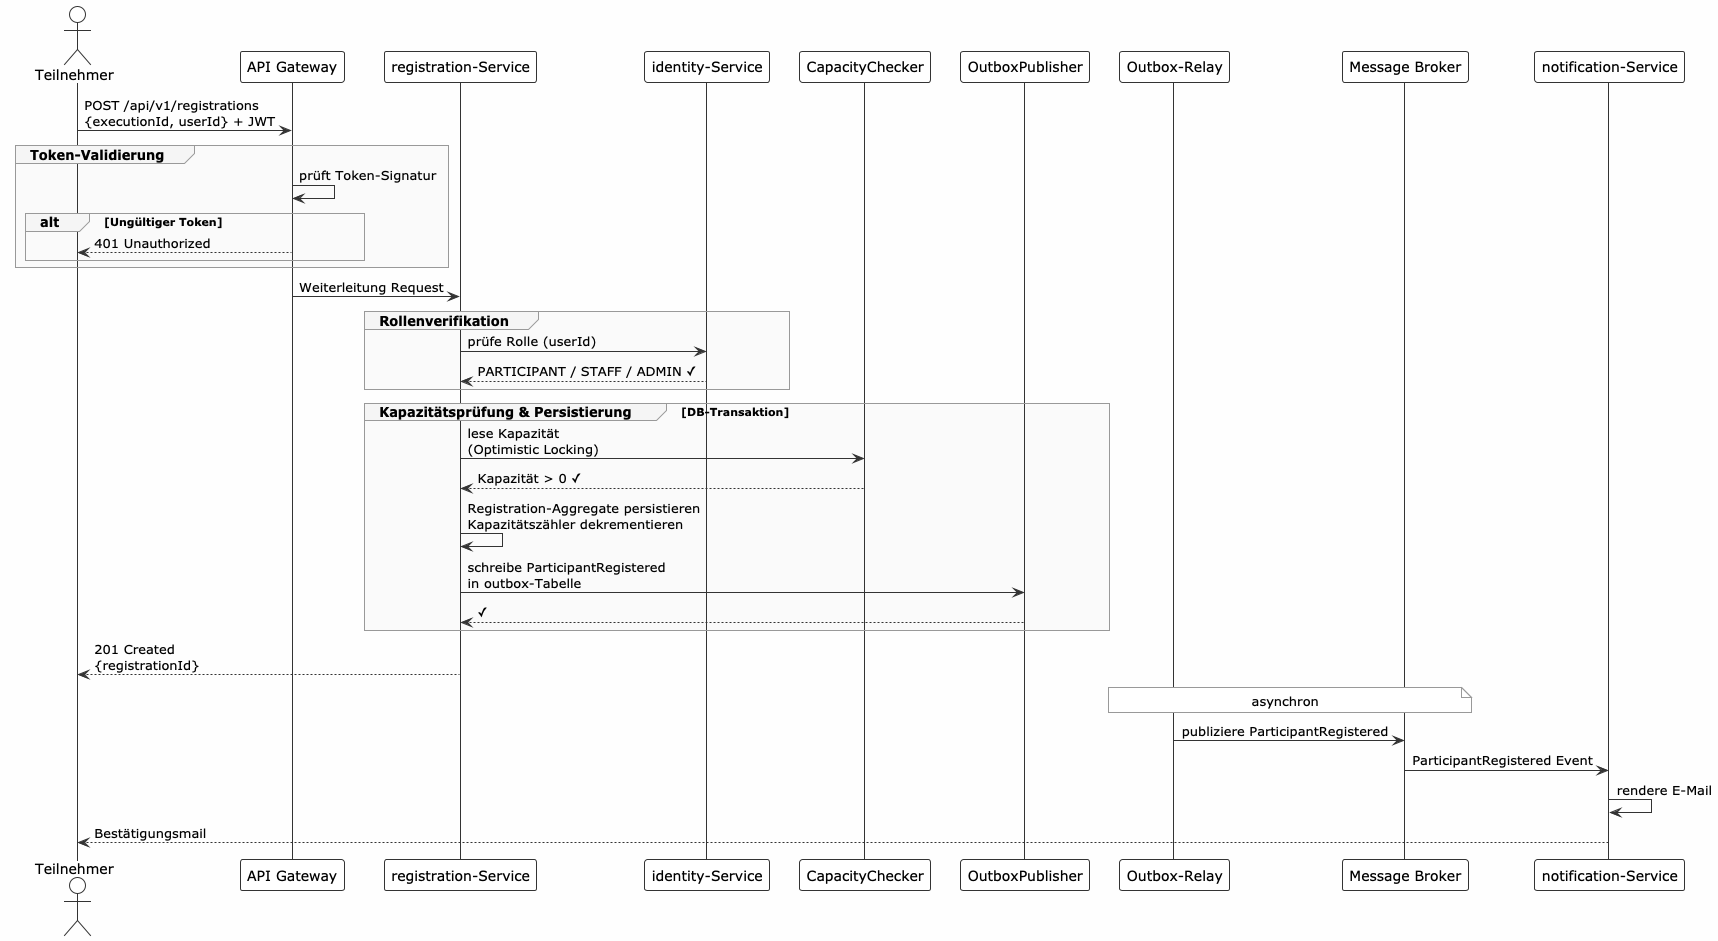
\includegraphics[width=\textwidth]{assets/sequence_diagram_1}
  \caption{\textit{Sequenz Diagramm für Teilnehmer schreibt sich ein (Happy Path)}}
  \label{fig:sequence_diagram_1}
\end{figure}


\subsection{Szenario~2: Kurs ausgebucht -- Warteliste}

Dieses Szenario behandelt den Fall, dass beim Einschreiben keine freie Kapazität mehr
vorhanden ist. Der Ablauf ist identisch mit Szenario~1 bis zur Kapazitätsprüfung;
anstelle einer Registrierung wird ein \texttt{WaitlistEntry} mit Zeitstempel und
Wartelisten-Position persistiert. Der Teilnehmer erhält eine \textbf{202~Accepted}-Antwort
sowie eine asynchrone Benachrichtigungsmail mit seiner Position.

Identisch mit Szenario~1 bis Schritt~5, dann:

\begin{enumerate}[leftmargin=2em, start=6]
  \item Kapazität = 0: WaitlistEntry mit Zeitstempel und nächster freier Position.
  \item Outbox-Event: \texttt{ParticipantAddedToWaitlist} (mit Position).
  \item Antwort: \textbf{202~Accepted} mit Wartelisten-Position.
\end{enumerate}


\begin{figure}[H]
  \centering
  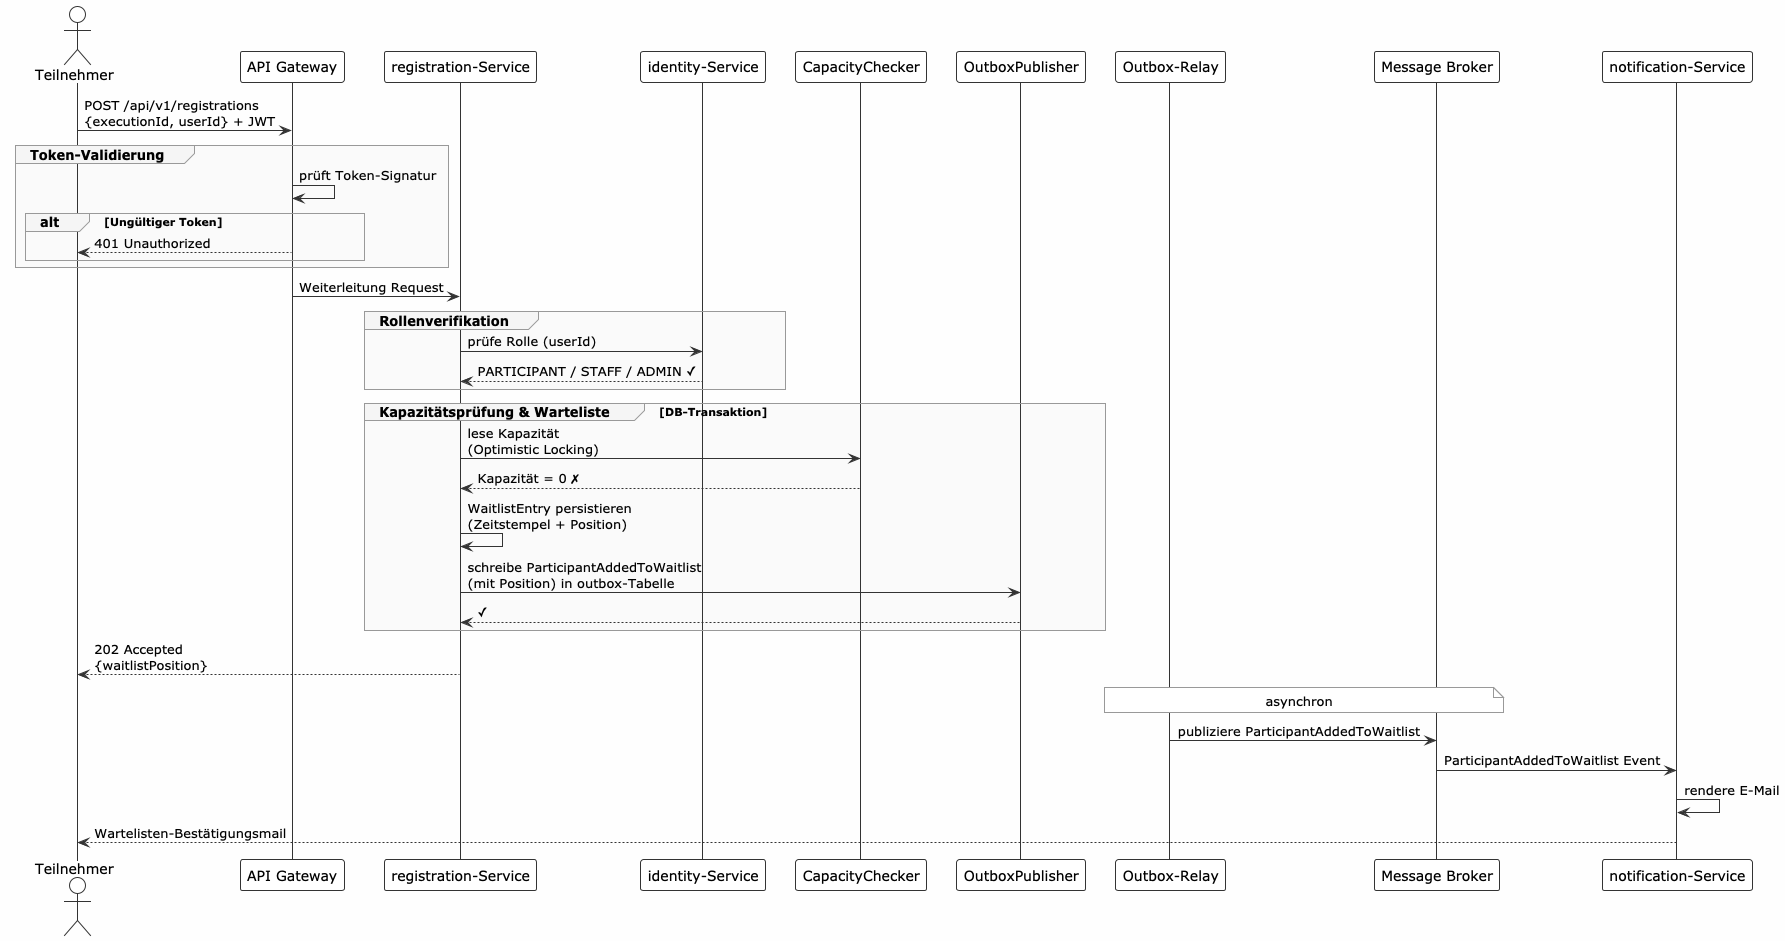
\includegraphics[width=\textwidth]{assets/sequence_diagram_2}
  \caption{\textit{Sequenz Diagramm für Teilnehmer schreibt sich ein, aber keine freien Plätze mehr }}
  \label{fig:sequence_diagram_2}
\end{figure}

\subsection{Szenario~3: Einschreibung stornieren}

Dieses Szenario beschreibt die Stornierung einer bestehenden Kursanmeldung. Nach der
Ownership-Prüfung -- nur eigene Einschreibungen dürfen storniert werden -- wird der
Status transaktional auf \texttt{CANCELLED} gesetzt und die Kapazität wieder freigegeben.
Ist die Warteliste nicht leer, rückt der älteste Eintrag automatisch nach; alle
Benachrichtigungen erfolgen asynchron über den \texttt{notification}-Service.

\begin{enumerate}[leftmargin=2em]
  \item \texttt{DELETE /api/v1/registrations/\{id\}} + JWT.
  \item Ownership-Prüfung: Nur eigene Einschreibungen dürfen storniert werden (403~Forbidden sonst).
  \item Status $\to$ CANCELLED; Kapazität inkrementiert.
  \item Outbox-Event: \texttt{RegistrationCancelled}.
  \item Falls Warteliste nicht leer: ältester Eintrag rückt nach $\to$ \texttt{WaitlistParticipantPromoted} + \texttt{ParticipantRegistered}.
  \item Antwort: \textbf{204~No~Content}.
\end{enumerate}

\begin{figure}[H]
  \centering
  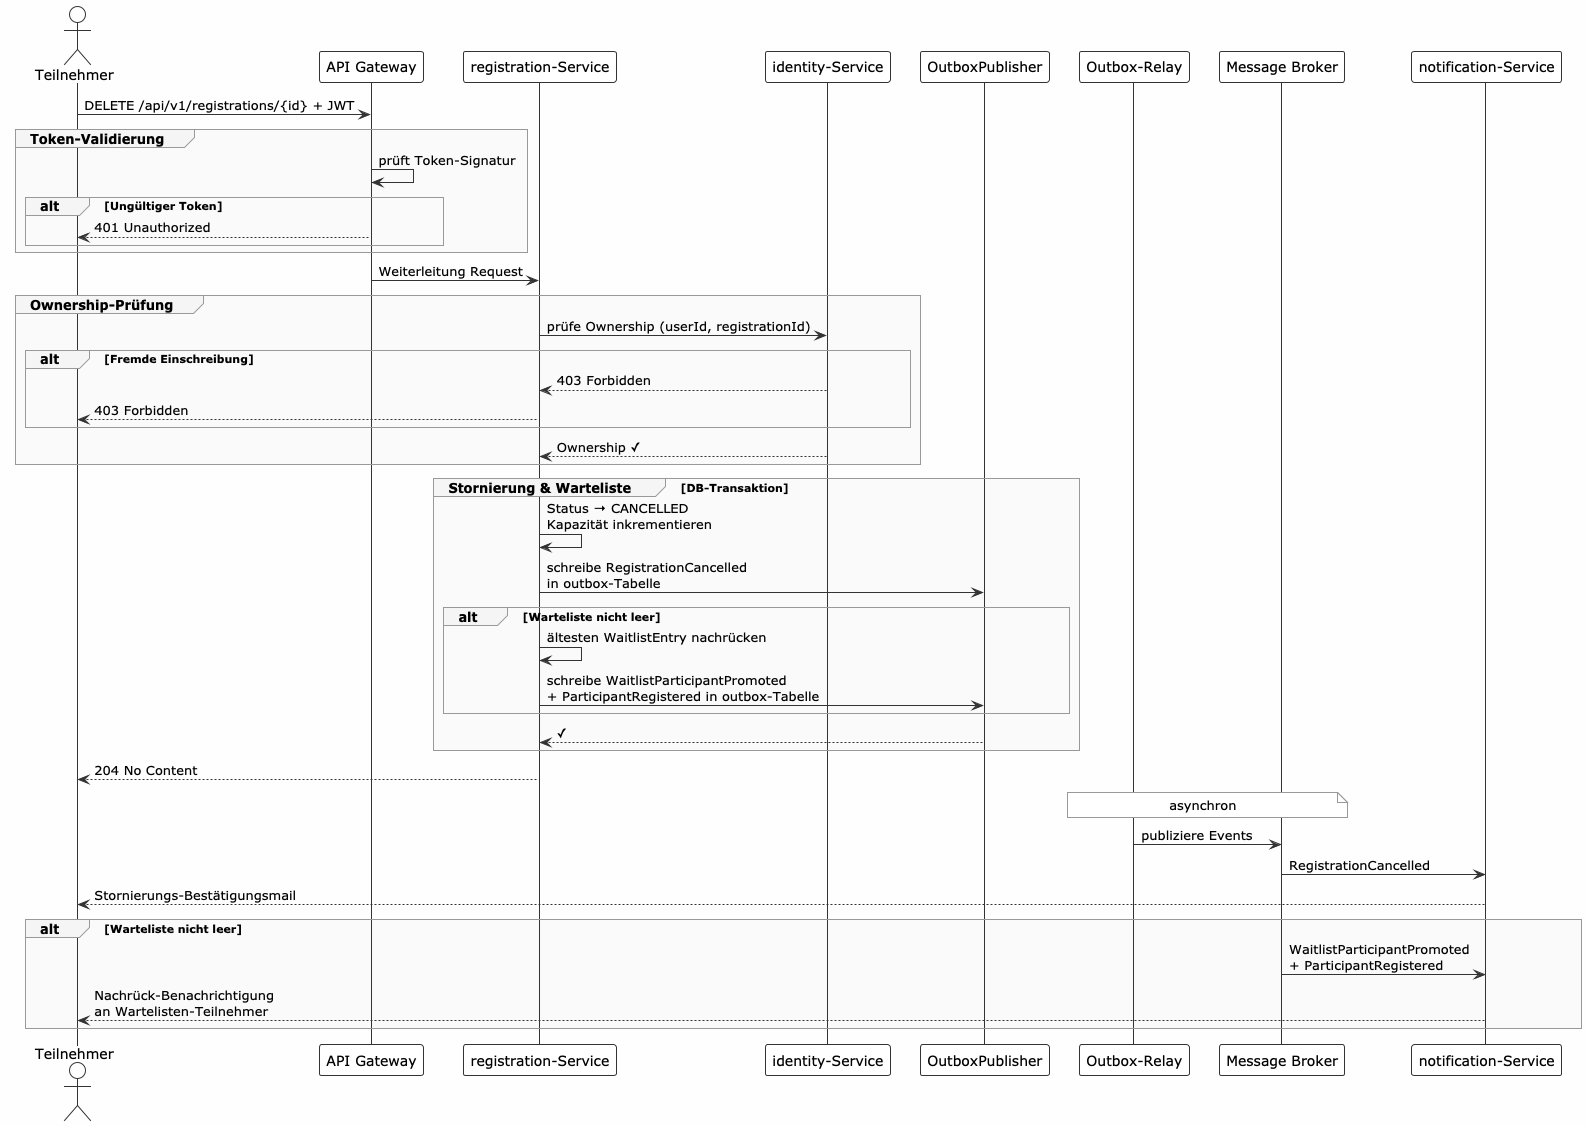
\includegraphics[width=\textwidth]{assets/sequence_diagram_3}
  \caption{\textit{Sequenz Diagramm für die Stornierung einer Kursanmeldung}}
  \label{fig:sequence_diagram_3}
\end{figure}

\subsection{Szenario~4: Admin veröffentlicht einen Kurs}

Dieses Szenario beschreibt die Veröffentlichung eines Kurses durch einen Administrator.
Der Ablauf ist bewusst schlank gehalten: Nach der Rollenprüfung -- ausschliesslich
ADMIN-Rolle ist berechtigt -- wird der \texttt{CourseStatus} transaktional von
\texttt{DRAFT} auf \texttt{PUBLISHED} gesetzt und das \texttt{CoursePublished}-Event
über die Outbox asynchron publiziert. Eine direkte Teilnehmer-Benachrichtigung
ist in diesem Szenario nicht vorgesehen.

\begin{enumerate}[leftmargin=2em]
  \item \texttt{PUT /api/v1/courses/\{id\}/publish} + JWT.
  \item ADMIN-Rolle erforderlich (403~Forbidden für alle anderen).
  \item \texttt{CourseStatus}: DRAFT $\to$ PUBLISHED.
  \item Outbox-Event: \texttt{CoursePublished}.
  \item Antwort: \textbf{200~OK}.
\end{enumerate}

\begin{figure}[H]
  \centering
  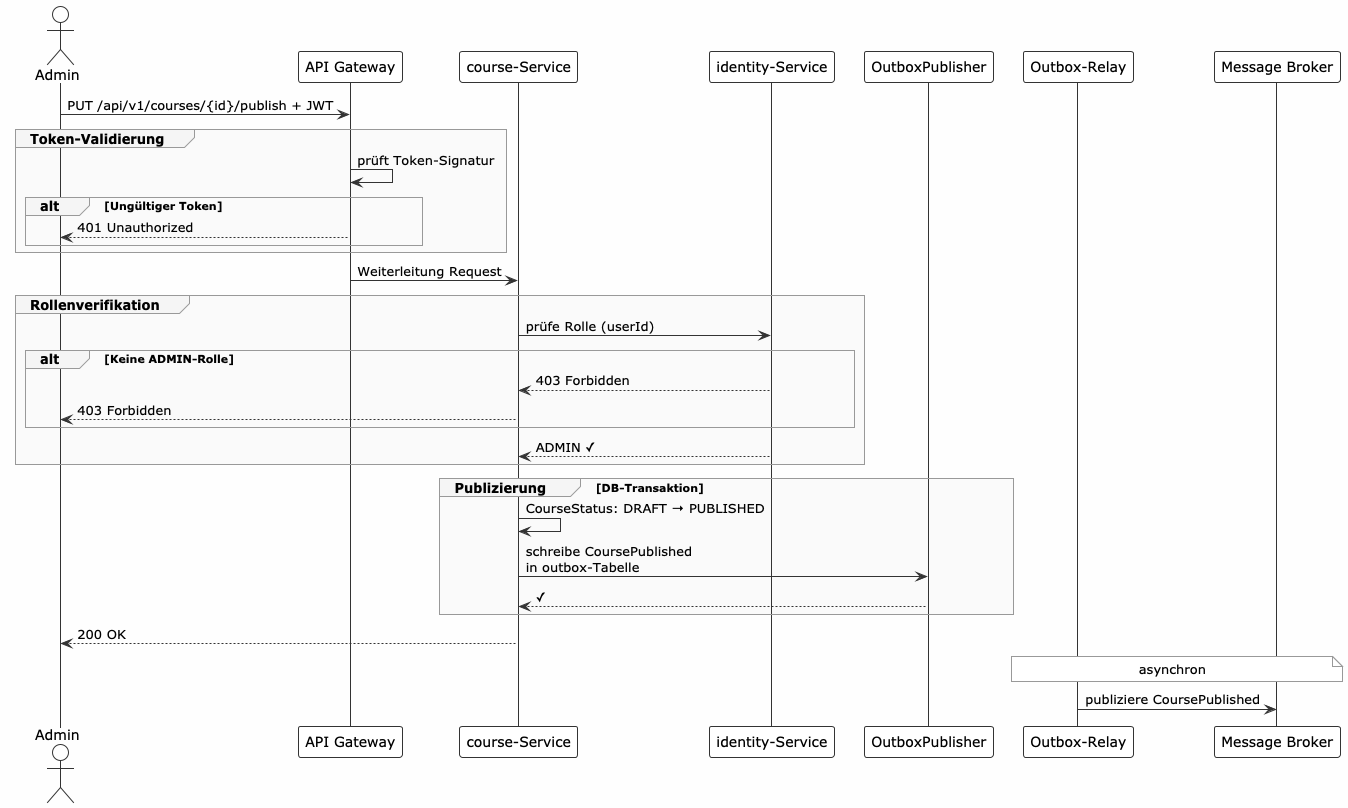
\includegraphics[width=\textwidth]{assets/sequence_diagram_4}
  \caption{\textit{Sequenz Diagramm für Admin veröffentlicht einen Kurs}}
  \label{fig:sequence_diagram_4}
\end{figure}


\subsection{Szenario~5: Cross-Context-Transaktion (Kurs archivieren)}

Dieses Szenario illustriert eine kontextübergreifende Transaktion, bei der das
Archivieren eines Kurses eine Kaskade von Zustandsänderungen in mehreren Services
auslöst. Da keine verteilte Transaktion verwendet wird, koordinieren sich
\texttt{catalog}, \texttt{scheduling}, \texttt{registration} und \texttt{notification}
ausschliesslich über Events -- die vollständige Konsistenz wird erst nach
$\sim$2--5~Sekunden erreicht (Eventual Consistency).

\begin{enumerate}[leftmargin=2em]
  \item \texttt{PUT /api/v1/courses/\{id\}/archive} (Admin).
  \item \texttt{catalog}: Status $\to$ ARCHIVED; Event \texttt{CourseArchived}.
  \item \texttt{scheduling} konsumiert $\to$ alle Executions $\to$ CANCELLED; Events \texttt{CourseExecutionCancelled}.
  \item \texttt{registration} konsumiert $\to$ alle Registrations $\to$ CANCELLED; Events \texttt{RegistrationCancelled}.
  \item \texttt{notification} versendet Massenstornierungsmails.
\end{enumerate}

\textit{Eventual Consistency:} Alle Services nach $\sim$2--5~Sek.\ konsistent.

\begin{figure}[H]
  \centering
  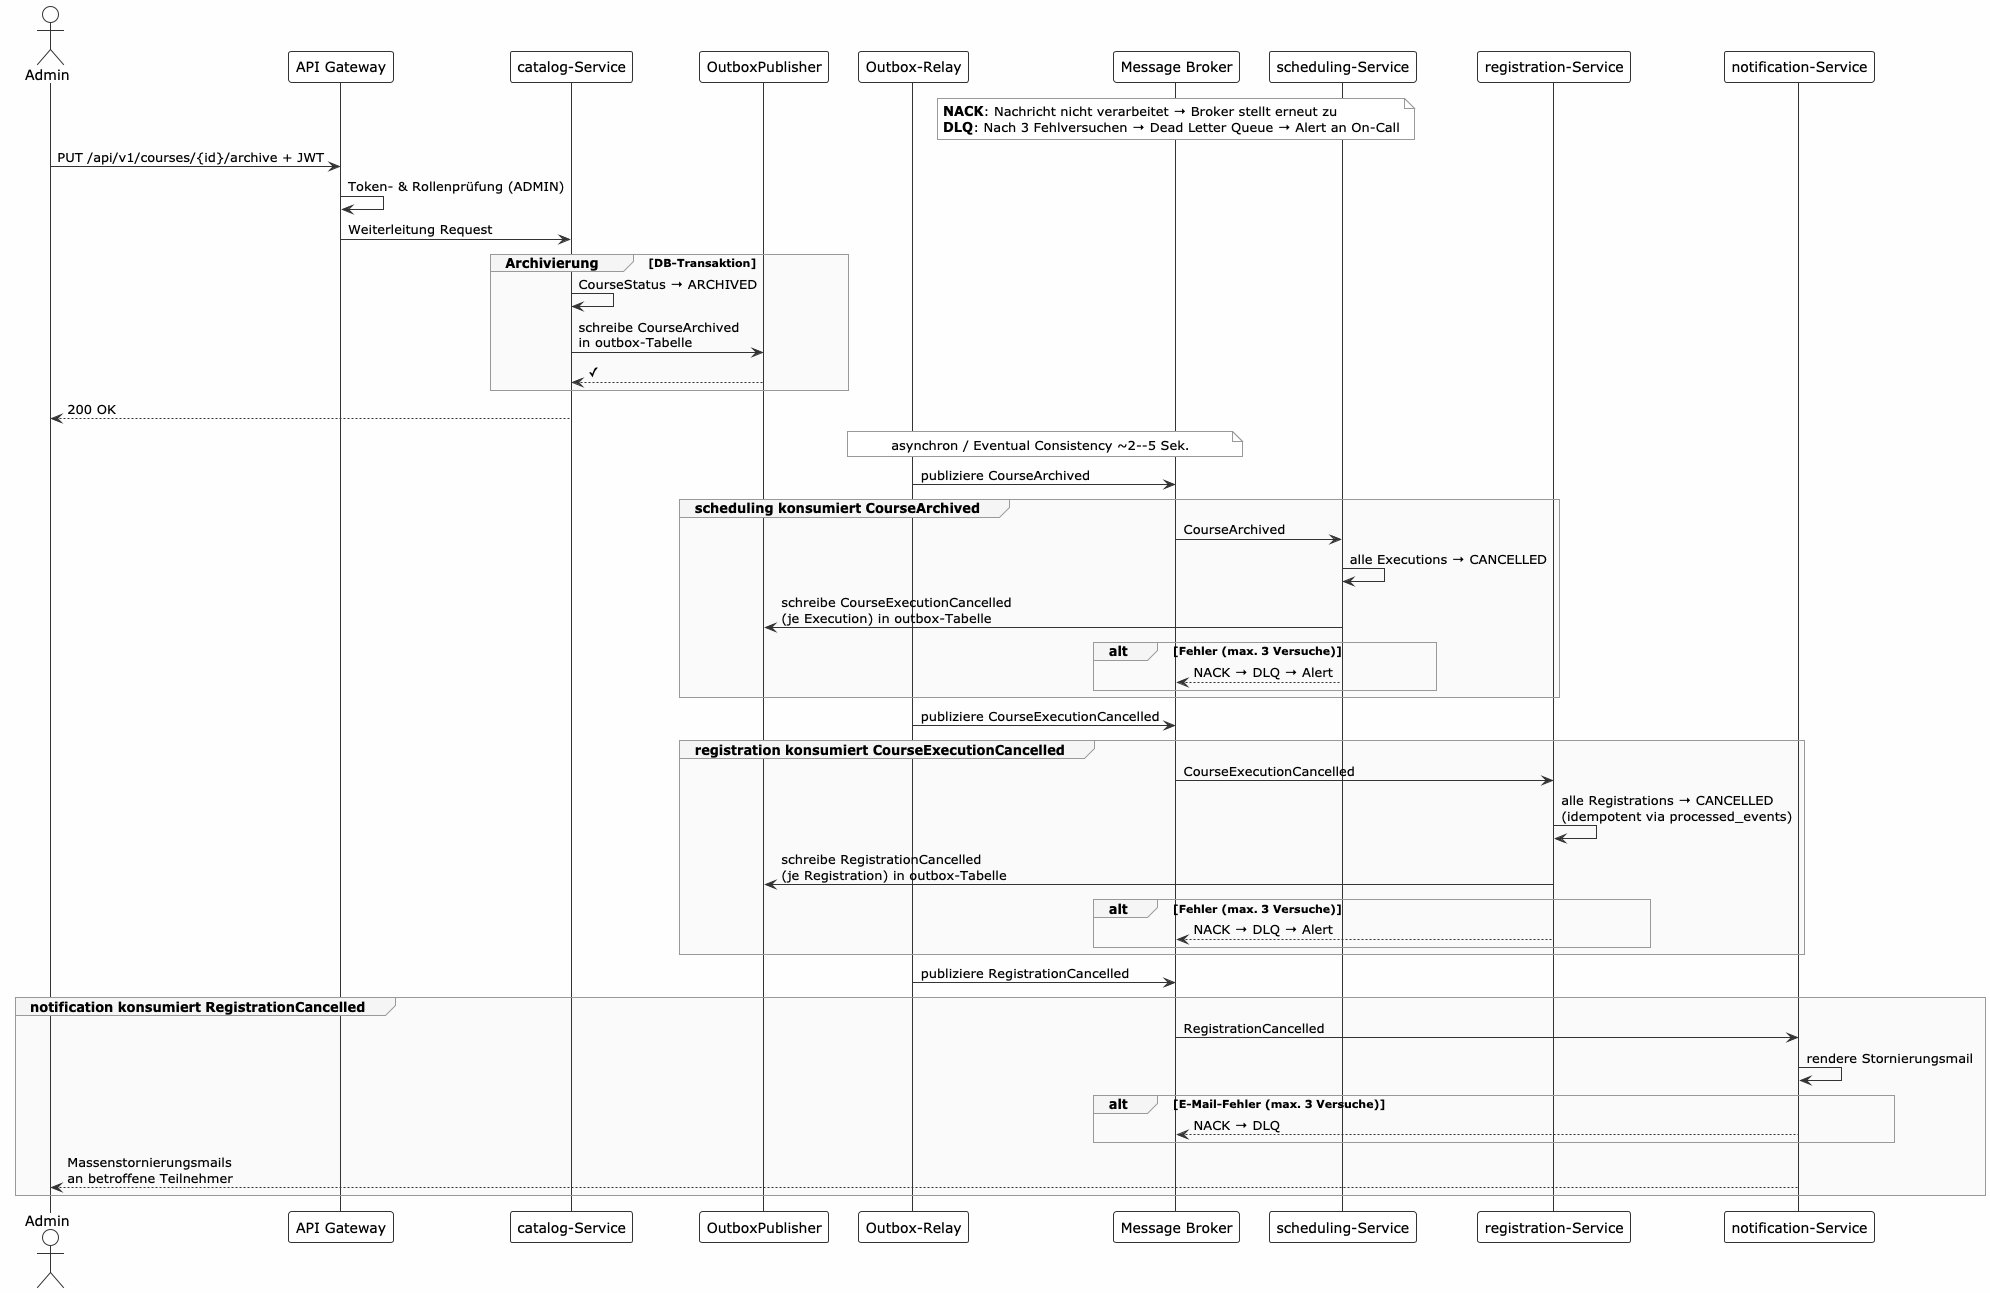
\includegraphics[width=\textwidth]{assets/sequence_diagram_5}
  \caption{\textit{Sequenz Diagramm für Kurs archivieren}}
  \label{fig:sequence_diagram_5}
\end{figure}

\begin{hinweis}[Fehlerbehandlung -- symmetrisch für alle Consumer]
  \textbf{Bei \texttt{registration}} (konsumiert \texttt{CourseExecutionCancelled}): Exception im Event-Handler $\to$
  RabbitMQ stellt erneut zu (at-least-once) $\to$ nach 3~Fehlversuchen DLQ $\to$ Alert $\to$ On-Call-Entwickler.
  Idempotenter Handler verhindert Doppelstornierungen.\\[4pt]
  \textbf{Bei \texttt{scheduling}} (konsumiert \texttt{CourseArchived}): Identischer DLQ-Mechanismus -- alle
  Executions werden auf CANCELLED gesetzt, sobald der Event erfolgreich verarbeitet ist.
  Idempotenz: \texttt{executionId} wird in \texttt{processed\_events}-Tabelle geprüft.\\[4pt]
  \textbf{Bei \texttt{notification}} (konsumiert \texttt{RegistrationCancelled}): Exception im E-Mail-Provider $\to$
  Retry (3x) $\to$ DLQ. Der Prozess (Einschreibung/Stornierung) ist bereits erfolgreich abgeschlossen.
\end{hinweis}